%% FullCourse_10Lecs -- Lecture 7, Act 1 (FRAME): Text as Economic Measurement
%% NEW deck (ch14 rebuild, 2026-07-07), per Lec07_ch14_Rebuild_Plan_2026-07-07.md.
%% Reused frames copied verbatim (with renumbered cross-references) from
%%   archive_pre_split/pre_ch14_rebuild_2026-07-07/Lec07_T1a_Why_LLMs_Tokenization.tex
%% New frames follow chapter14 (Book1) sec. 14.1: text-DGP spine, EPU/FOMC/PRisk
%% case unit, feasibility window, China parallels.

%% Shared preamble for the FullCourse_10Lecs topic decks.
%%
%% Each topic .tex \input's this file, then defines its own \title, \date
%% override (if any), \graphicspath, and \begin{document}.
%%
%% Reconstructed verbatim from the inlined copy preserved in
%% Lec10_Case_Studies/Lec10_T8_Case6_DeepRamsey.tex (lines 23-190), which is
%% explicitly annotated there as "from ../shared_preamble.tex, copied verbatim".
%% Base preamble matches MiniCourse_8hr/Slides/shared_preamble.tex; this version
%% additionally provides \sectiondivider, the conceptbox/cautionbox/examplebox/
%% takeawaybox tcolorboxes, and \compacttables used across the split decks.

\documentclass[10pt,english,aspectratio=169]{beamer}

\usepackage{ae,aecompl}
\usepackage[T1]{fontenc}
\usepackage{textcomp}
\usepackage[utf8]{inputenc}
\usepackage{babel}
\usepackage{datetime2}

\setcounter{secnumdepth}{3}
\setcounter{tocdepth}{3}

\usepackage{amsmath, amssymb, amsthm, graphicx}
\usepackage{booktabs, multirow}
\usepackage{tikz}
\usepackage{pgfplots}
\pgfplotsset{compat=1.16}
\usepackage[most]{tcolorbox}
\tcbuselibrary{skins, breakable, theorems}
\usepackage{listings}
\usepackage{xcolor}

\lstset{
  basicstyle=\ttfamily\small,
  keywordstyle=\color{blue!80!black}\bfseries,
  commentstyle=\color{green!50!black}\itshape,
  stringstyle=\color{orange!80!black},
  backgroundcolor=\color{gray!8},
  frame=single,
  rulecolor=\color{gray!40},
  breaklines=true,
  showstringspaces=false,
  numbers=none,
}

\lstdefinestyle{pythonstyle}{
    language=Python,
    basicstyle=\ttfamily\footnotesize,
    keywordstyle=\color{blue!80!black}\bfseries,
    commentstyle=\color{green!50!black}\itshape,
    stringstyle=\color{orange!80!black},
    frame=single,
    breaklines=true,
    showstringspaces=false,
    numbers=left,
    numbersep=5pt,
    numberstyle=\tiny\color{gray},
    backgroundcolor=\color{gray!8},
    rulecolor=\color{gray!40}
}

\ifx\hypersetup\undefined
  \AtBeginDocument{%
    \hypersetup{bookmarks=false,breaklinks=true,pdfborder={0 0 0},colorlinks=true,
      linkcolor=DarkText,urlcolor=RedTitle}%
  }
\else
  \hypersetup{bookmarks=false,breaklinks=true,pdfborder={0 0 0},colorlinks=true,
    linkcolor=DarkText,urlcolor=RedTitle}%
\fi

\makeatletter
\newcommand\makebeamertitle{%
  \begin{frame}[plain]
    \vspace*{1.0cm}
    \centering
    {\usebeamerfont{title}\usebeamercolor[fg]{title}\inserttitle\par}
    \vspace{1.0cm}
    {\usebeamerfont{author}\usebeamercolor[fg]{author}\insertauthor\par}
    \vspace{0.2cm}
    {\usebeamerfont{date}\usebeamercolor[fg]{date}\insertdate\par}
  \end{frame}}%
\AtBeginDocument{%
  \let\origtableofcontents=\tableofcontents
  \def\tableofcontents{\@ifnextchar[{\origtableofcontents}{\gobbletableofcontents}}
  \def\gobbletableofcontents#1{\origtableofcontents}%
}

\usetheme{metropolis}
\usefonttheme{professionalfonts}

\definecolor{LightGray}{RGB}{230,230,230}
\definecolor{RedTitle}{RGB}{0,0,200}
\definecolor{VeryLightGray}{RGB}{245,245,245}
\definecolor{DarkText}{RGB}{0,0,0}

\setbeamercolor{background canvas}{bg=white}
\setbeamercolor{title}{fg=RedTitle}
\setbeamercolor{author}{fg=DarkText}
\setbeamercolor{date}{fg=DarkText}
\setbeamercolor{frametitle}{bg=VeryLightGray,fg=DarkText}
\setbeamercolor{normal text}{fg=DarkText}
\setbeamerfont{title}{size=\large}

\setbeamersize{text margin left=5mm, text margin right=5mm}
\addtobeamertemplate{frametitle}{}{\vspace{-0.5em}}
\newcommand{\reducevspace}{\vspace{-0.5cm}}

% Shared section divider and box styles for split topic decks.
\newcommand{\sectiondivider}[2]{%
\begin{frame}[plain,noframenumbering]
\begin{center}
\vfill
{\Large\textbf{#1}\par}
\vspace{0.35cm}
{\normalsize #2\par}
\vfill
\end{center}
\end{frame}
}

\newtcolorbox{conceptbox}[1][]{
  colback=blue!3,
  colframe=RedTitle!55,
  boxrule=0.35mm,
  arc=1mm,
  left=2mm,
  right=2mm,
  top=1mm,
  bottom=1mm,
  #1
}
\newtcolorbox{cautionbox}[1][]{
  colback=red!3,
  colframe=red!50!black,
  boxrule=0.35mm,
  arc=1mm,
  left=2mm,
  right=2mm,
  top=1mm,
  bottom=1mm,
  #1
}
\newtcolorbox{examplebox}[1][]{
  colback=green!3,
  colframe=green!45!black,
  boxrule=0.35mm,
  arc=1mm,
  left=2mm,
  right=2mm,
  top=1mm,
  bottom=1mm,
  #1
}
\newtcolorbox{takeawaybox}[1][]{
  colback=VeryLightGray,
  colframe=RedTitle!55,
  boxrule=0.35mm,
  arc=1mm,
  left=2mm,
  right=2mm,
  top=1mm,
  bottom=1mm,
  #1
}
\newcommand{\compacttables}{\renewcommand{\arraystretch}{1.15}}

\setbeamertemplate{navigation symbols}{}
\setbeamertemplate{footline}{%
  \hfill%
  \usebeamercolor[fg]{page number in head/foot}%
  \usebeamerfont{page number in head/foot}%
  \insertframenumber\,/\,\inserttotalframenumber\kern1em\vskip2pt%
}

\makeatother

\author{Zhigang Feng}
% "date with time": compile timestamp so each build is identifiable.
\date{\today\ \DTMcurrenttime}


% Suppress redundant auto-generated metropolis section page; \sectiondivider frames are the dividers we keep.
\metroset{sectionpage=none}

\graphicspath{{./pic/}{../../MiniCourse_8hr/Slides/Module3_LLM_Text/pic/}{../}}

\usetikzlibrary{arrows.meta,positioning,shapes,calc,fit,backgrounds}

%% Lec07 shared MAP slide: "one map, five acts" recurring diagram.
%% Adapted from ../Lec09_Agentic_AI/lec09_map.tex (\LecNineMap -> \LecSevenMap).
%% Input this file AFTER ../shared_preamble.tex (needs RedTitle, VeryLightGray)
%% and call \LecSevenMap{k} inside a frame, where k in {1..5} highlights the
%% current act ("you are here") and k = 0 renders the closing reprise with all
%% five acts complete (used by T5b's closing frame).
%% Filename deliberately does not match the build glob Lec*_T*.tex, so the
%% build script never tries to compile it standalone.

\newcommand{\LecSevenMap}[1]{%
% Precompute per-box style selectors; TikZ option lists are comma-split before
% TeX conditionals run, so \ifnum must not sit inside a [...] options list.
\ifnum#1=0
  \tikzset{lecmapa/.style={lecmapdone}, lecmapb/.style={lecmapdone},
           lecmapc/.style={lecmapdone}, lecmapd/.style={lecmapdone},
           lecmape/.style={lecmapdone}}%
\else
  \tikzset{lecmapa/.style={}, lecmapb/.style={}, lecmapc/.style={},
           lecmapd/.style={}, lecmape/.style={}}%
  \ifnum#1=1 \tikzset{lecmapa/.style={lecmapcur}}\fi
  \ifnum#1=2 \tikzset{lecmapb/.style={lecmapcur}}\fi
  \ifnum#1=3 \tikzset{lecmapc/.style={lecmapcur}}\fi
  \ifnum#1=4 \tikzset{lecmapd/.style={lecmapcur}}\fi
  \ifnum#1=5 \tikzset{lecmape/.style={lecmapcur}}\fi
\fi
\begin{center}
\begin{tikzpicture}[
    act/.style={rectangle, rounded corners, draw=black!60, fill=VeryLightGray,
        minimum width=2.6cm, minimum height=0.92cm, text width=2.5cm,
        align=center, font=\scriptsize, text=DarkText},
    lecmapcur/.style={draw=RedTitle, very thick, fill=orange!20},
    lecmapdone/.style={draw=green!45!black, thick, fill=green!10},
    q/.style={font=\tiny\itshape, text width=2.7cm, align=center, text=black!70},
    sat/.style={rectangle, rounded corners, draw=black!45, dashed, fill=white,
        text width=5.0cm, align=center, font=\tiny, text=black!70,
        minimum height=0.5cm},
    barlab/.style={font=\tiny\bfseries, text=black!60},
    arr/.style={-{Stealth[length=2mm]}, thick, gray!60}
]
    % --- five act boxes ---
    \node[act, lecmapa] (a1) at (0,0)
        {\textbf{7.1 FRAME}\\ \tiny text as measurement};
    \node[act, lecmapb] (a2) at (2.85,0)
        {\textbf{7.2 REPRESENT}\\ \tiny tokens $\to$ vectors};
    \node[act, lecmapc] (a3) at (5.7,0)
        {\textbf{7.3 ATTEND}\\ \tiny attention \& Transformer};
    \node[act, lecmapd] (a4) at (8.55,0)
        {\textbf{7.4 PRETRAIN}\\ \tiny LMs \& alignment};
    \node[act, lecmape] (a5) at (11.4,0)
        {\textbf{7.5 MEASURE}\\ \tiny limits, apps, validation};
    \draw[arr] (a1) -- (a2);
    \draw[arr] (a2) -- (a3);
    \draw[arr] (a3) -- (a4);
    \draw[arr] (a4) -- (a5);
    % --- the student question each act answers ---
    \node[q] at (0,-0.82)    {what generates\\ this text?};
    \node[q] at (2.85,-0.82) {how do we turn it\\ into numbers?};
    \node[q] at (5.7,-0.82)  {how does context\\ get encoded?};
    \node[q] at (8.55,-0.82) {where does a pretrained\\ model come from?};
    \node[q] at (11.4,-0.82) {is my measure valid ---\\ and defensible?};
    % --- "you are here" marker above the current act ---
    \ifnum#1=1 \node[font=\scriptsize\bfseries, text=RedTitle] at (0,0.95)
        {you are here\ $\blacktriangledown$};\fi
    \ifnum#1=2 \node[font=\scriptsize\bfseries, text=RedTitle] at (2.85,0.95)
        {you are here\ $\blacktriangledown$};\fi
    \ifnum#1=3 \node[font=\scriptsize\bfseries, text=RedTitle] at (5.7,0.95)
        {you are here\ $\blacktriangledown$};\fi
    \ifnum#1=4 \node[font=\scriptsize\bfseries, text=RedTitle] at (8.55,0.95)
        {you are here\ $\blacktriangledown$};\fi
    \ifnum#1=5 \node[font=\scriptsize\bfseries, text=RedTitle] at (11.4,0.95)
        {you are here\ $\blacktriangledown$};\fi
    \ifnum#1=0 \node[font=\scriptsize\bfseries, text=green!45!black] at (5.7,0.95)
        {all five acts complete};\fi
    % --- bottom band: the measurement sandwich ---
    \fill[blue!10]   (-1.3,-1.55) rectangle (1.40,-1.22);
    \fill[green!10]  (1.65,-1.55) rectangle (9.85,-1.22);
    \fill[orange!15] (10.1,-1.55) rectangle (12.7,-1.22);
    \node[barlab] at (0.05,-1.385) {WHY TEXT = MEASUREMENT};
    \node[barlab] at (5.75,-1.385) {HOW THE MACHINE READS TEXT};
    \node[barlab] at (11.4,-1.385) {MEASURE, VALIDATE, DISCLOSE};
    % --- the recurring spine (text DGP), printed under the band ---
    \node[font=\tiny\itshape, text=black!60] at (5.7,-1.83)
        {the spine:\ \ $x_i = g(s_i,\,a_i,\,c_i)+\varepsilon_i
         \;\longrightarrow\; m(x_i)
         \;\longrightarrow\; y_i = \beta\,m(x_i)+\gamma z_i+u_i$};
    % --- dashed satellites: the neighbouring lectures ---
    \node[sat] at (2.0,-2.42)
        {\textit{before 7.1:} Lec03--04 gave you neural nets, backprop \& PyTorch --- Lec07 teaches them to read};
    \node[sat] at (9.8,-2.42)
        {\textit{after 7.5:} Lec08 RAG (grounded memory) $\to$ Lec09 agents (grounded action) $\to$ Lec10 cases};
\end{tikzpicture}
\end{center}
}


\title[AI for Econ Research]{AI for Economic Research: Dynamic Models, Language, and Agents\\
Lecture 7.1: Text as Economic Measurement}

\begin{document}

\makebeamertitle

%=============================================================================
\begin{frame}{Lecture 7 in One Map}
\LecSevenMap{1}
\medskip
\textit{\footnotesize Two case threads run through all five acts --- \textbf{Thread A: the EPU index} (Baker--Bloom--Davis 2016), the transparent dictionary baseline every method must beat; \textbf{Thread B: FOMC hawk--dove} (central-bank communication), the running example for embeddings, attention, and validation. Watch for them.}
\end{frame}

%=============================================================================
\section{Text as Data}
\sectiondivider{Text as Data}{Why language became an economic measurement problem}

\begin{frame}{The Opening Hook: Reading Uncertainty out of Newspapers}
\textbf{In 2016, three economists asked: can you \emph{read} policy uncertainty out of the newspaper?}
\begin{itemize}
\item Baker, Bloom \& Davis (2016, \emph{QJE}): scan 10 major US newspapers, month by month, and count articles containing \textbf{all three} of \{\texttt{economic}/\texttt{economy}\}, \textbf{and} \{\texttt{uncertain}/\texttt{uncertainty}\}, \textbf{and} one of \{\texttt{Congress}, \texttt{deficit}, \texttt{Federal Reserve}, \texttt{legislation}, \texttt{regulation}, \texttt{White House}\}.
\item Scale by each paper's total output, standardize, average across papers, index to 100:
\[
   \mathrm{EPU}_\tau \;=\; 100 \times \frac{u_\tau}{\bar u}, \qquad
   u_\tau \;=\; \frac{1}{10}\sum_{p=1}^{10}\frac{c_{p\tau}/N_{p\tau}}{\sigma_p}.
\]
{\scriptsize where $p=1,\dots,10$ indexes newspapers, $\tau$ the month; $c_{p\tau}$ = qualifying articles in paper $p$; $N_{p\tau}$ = paper $p$'s total articles (dividing removes size differences); $\sigma_p$ = std.\ dev.\ of paper $p$'s scaled series (so no one paper dominates); $u_\tau$ = 10-paper average; $\bar u$ = its sample mean, so $\times100$ sets the average to 100.}
\item No statistical agency publishes ``policy uncertainty'' --- it is not directly observed anywhere. Yet in a VAR, EPU spikes precede investment and employment declines.
\end{itemize}
\smallskip
\textbf{The move that matters:} unstructured language became a \emph{regression-ready variable} --- this act asks what that takes, and where it goes wrong. \textit{(Thread A begins.)}
\end{frame}

\begin{frame}{Text as Economic Data --- The Big Picture}
\centering
\begin{tikzpicture}[
  every node/.style={font=\scriptsize},
  src/.style={draw, rounded corners=1pt, minimum width=28mm, minimum height=6mm, fill=blue!12, align=center},
  rep/.style={draw, rounded corners=1pt, minimum width=30mm, minimum height=6mm, fill=orange!18, align=center},
  outcome/.style={draw, rounded corners=1pt, minimum width=30mm, minimum height=6mm, fill=green!18, align=center},
  arr/.style={-{Latex[length=1.5mm]}, thick}
]
% Sources column
\node[font=\small\bfseries] (h1) at (0,2.6) {Raw text sources};
\node[src] (s1) at (0,1.8)  {FOMC minutes \& speeches};
\node[src] (s2) at (0,0.9)  {SEC EDGAR 10-K, MD\&A};
\node[src] (s3) at (0,0.0)  {News, earnings calls};
\node[src] (s4) at (0,-0.9) {Patents, congressional records};

% Representation column
\node[font=\small\bfseries] (h2) at (5.5,2.6) {Representation};
\node[rep] (r1) at (5.5,1.4) {Counts (TF-IDF, dictionaries)};
\node[rep] (r2) at (5.5,0.5) {Static embeddings (W2V, GloVe)};
\node[rep] (r3) at (5.5,-0.4) {Contextual (BERT, GPT, Claude)};

% Outcome column
\node[font=\small\bfseries] (h3) at (11,2.6) {Economic / business variables};
\node[outcome] (o1) at (11,1.7) {Uncertainty / sentiment indices};
\node[outcome] (o2) at (11,0.8) {Firm risk, exposure, similarity};
\node[outcome] (o3) at (11,-0.1) {Stance, narrative shifts};
\node[outcome] (o4) at (11,-1.0) {Forecasts / nowcasts};

% Arrows source -> rep
\foreach \s in {s1,s2,s3,s4}{ \draw[arr, gray!60] (\s.east) -- ($(r2.west)+(-0.1,0)$); }
% Arrows rep -> outcome
\foreach \r in {r1,r2,r3}{ \draw[arr, gray!60] (\r.east) -- ($(o2.west)+(-0.1,0)$); }
\end{tikzpicture}

\medskip
{\footnotesize\textit{The lecture builds the middle column rung by rung: Act 2 counts $\to$ static embeddings, Act 3 contextual machinery, Act 4 how those models are trained --- and Act 5 turns the machinery into the right-hand column, with validation.}}
\end{frame}

\begin{frame}{Why Economists Care About LLMs}
\begin{itemize}
\item \textbf{Text as data} --- modern economic research increasingly leverages textual sources:
\begin{itemize}
    \item Corporate filings (10-K, 10-Q, MD\&A)
    \item Central bank speeches, FOMC minutes, ECB statements
    \item Earnings calls, analyst reports, regulatory filings
    \item News, social media, congressional records
\end{itemize}

\medskip
\item \textbf{Applications:}
\begin{itemize}
    \item Sentiment analysis for financial forecasting
    \item Policy stance detection and uncertainty indices
    \item New text-derived macroeconomic indicators
    \item Summarization of long, technical documents
\end{itemize}

\medskip
\item \textbf{Why LLMs in particular:}
\begin{itemize}
    \item Capture nuanced language and domain-specific jargon
    \item Handle long-range context (sentences, paragraphs, whole documents)
    \item Provide a unified architecture for many tasks
\end{itemize}
\end{itemize}
\end{frame}

\begin{frame}{Three Roles of Text in Economic Research}
\begin{center}
\renewcommand{\arraystretch}{1.35}
\begin{tabular}{l p{4cm} p{6cm}}
\toprule
\textbf{Role} & \textbf{What text is} & \textbf{Example} \\
\midrule
Measurement tool & A way to construct previously unobserved variables & Baker--Bloom--Davis (2016) Economic Policy Uncertainty index from newspapers \\
Behavioral outcome & A response variable revealing decisions or institutional change & Hansen, McMahon \& Prat (2018): how FOMC transparency reform changed committee speech \\
Treatment variable & A quasi-experimental input affecting behavior & Central bank communication shocks and inflation expectations \\
\bottomrule
\end{tabular}
\end{center}

\end{frame}

\begin{frame}{Why Now? The Feasibility Window}
\textbf{Two curves crossed around 2017: the cost of handling text collapsed while model capability exploded.}
\begin{center}
\begin{tikzpicture}[font=\scriptsize, xscale=0.78, yscale=0.55]
% feasible region
\fill[green!8] (7.44,0) rectangle (12.4,6);
\node[font=\tiny, green!45!black, align=center, text width=3.0cm] at (10.1,5.5)
    {text measurement becomes\\ a routine research tool};
% axes
\draw[-{Latex[length=2mm]}, gray!60] (0,0) -- (13.0,0) node[below left, font=\tiny, black] {year};
\draw[-{Latex[length=2mm]}, gray!60] (0,0) -- (0,6.2);
\foreach \x/\yr in {0.6/2008, 4.4/2013, 7.44/2017, 9.72/2020, 12.0/2023} {
    \draw[gray!45] (\x,0.07) -- (\x,-0.07);
    \node[font=\tiny, gray!50!black, below] at (\x,-0.06) {\yr};
}
% cost curve (disk $/GB, log scale, stylized through real points)
\draw[very thick, red!65] plot[smooth, tension=0.55] coordinates
    {(0.6,5.5) (4.4,3.6) (7.44,2.6) (9.72,1.6) (12.0,1.0)};
\node[font=\tiny, red!55!black, anchor=west] at (0.75,5.6) {$\approx\$0.30$/GB};
\node[font=\tiny, red!55!black, anchor=west] at (10.3,1.1) {$\approx\$0.01$/GB};
% capability curve (model parameters, log scale)
\draw[very thick, blue!70] plot[smooth, tension=0.55] coordinates
    {(0.6,0.55) (4.4,1.3) (7.44,2.5) (8.4,3.2) (9.72,4.7) (12.0,5.3)};
% legend
\draw[very thick, red!65] (1.0,2.6)--(1.55,2.6);
\node[anchor=west, font=\tiny, red!55!black] at (1.6,2.6) {storage cost (\$/GB) $\downarrow$};
\draw[very thick, blue!70] (1.0,2.05)--(1.55,2.05);
\node[anchor=west, font=\tiny, blue!55!black] at (1.6,2.05) {model scale (parameters) $\uparrow$};
% crossing threshold
\draw[dashed, gray!55] (7.44,0) -- (7.44,2.5);
% milestones
\fill[blue!70] (4.4,1.3) circle (1.5pt);
\node[font=\tiny, blue!55!black, below, align=center] at (4.4,1.12) {Word2Vec\\ 2013};
\fill[blue!70] (7.44,2.5) circle (1.5pt);
\node[font=\tiny, blue!55!black, align=center] at (6.35,3.25) {Transformer 2017\\ (65M params)};
\fill[blue!70] (8.4,3.2) circle (1.5pt);
\node[font=\tiny, blue!55!black, align=center] at (7.55,4.25) {BERT 2018\\ (340M)};
\fill[blue!70] (9.72,4.7) circle (1.5pt);
\node[font=\tiny, blue!55!black, anchor=west] at (9.95,4.5) {GPT-3 2020 (175B)};
\end{tikzpicture}
\end{center}
{\footnotesize\textit{Both quantities on log scales; curves are stylized interpolations through the marked real data points. Storage costs after McCallum's disk-price series; model sizes from Vaswani et al.\ (2017), Devlin et al.\ (2018), Brown et al.\ (2020).}}
\end{frame}

%=============================================================================
\section{The Spine}
\sectiondivider{The Spine}{A data-generating process for text --- and the two hazards it creates}

\begin{frame}{An Identification-First View of Text}
\begin{itemize}
\item \textbf{Engineering perspective first:} to a machine, a document is just a character string. But every string was \emph{produced} --- by a person, in a situation, for an audience. Before any econometrics, ask: what generated this string?

\medskip
\item \textbf{The data-generating process (DGP):}
\[
   x_i \;=\; g\bigl(s_i,\; a_i,\; c_i\bigr) \;+\; \varepsilon_i
\]
\begin{itemize}
    \item $s_i$: the latent \textbf{economic state} we want to measure (policy stance, sentiment, firm risk)
    \item $a_i$: the speaker's \textbf{strategic framing} --- audience management, spin, emphasis, tone chosen for effect
    \item $c_i$: \textbf{institutional context} --- venue, legal disclosure requirements, format conventions
\end{itemize}

\medskip
\item \textbf{Why this matters for a downstream regression} $y_i = \beta\,m(x_i) + \gamma z_i + u_i$: if the strategic framing $a_i$ is correlated with the regression error $u_i$, then the text feature $m(x_i)$ is \emph{endogenous} --- the familiar omitted-variable problem, now hidden inside the language.
\end{itemize}
\end{frame}

\begin{frame}{Two Firms, Same Risk, Different Words}
\textbf{The endogeneity hazard, made concrete.} Imagine two firms facing the \emph{same} objective political risk $s_i$.
\medskip
\begin{cautionbox}
\begin{itemize}
\item Firm A's management discloses risks proactively --- building a reputation for transparency.
\item Firm B's management avoids politically sensitive topics --- afraid of spooking the market.
\item Same $s_i$, different strategic framing $a_i$ $\;\Rightarrow\;$ different texts $x_i$ $\;\Rightarrow\;$ different measured risk $m(x_i)$.
\end{itemize}
\end{cautionbox}
\medskip
\begin{itemize}
\item If the disclosure choice $a_i$ correlates with anything in $u_i$ (governance quality, investor base, financial health), $m(x_i)$ is \textbf{endogenous} --- before any fancy NLP even enters.
\end{itemize}
\smallskip
\textit{\footnotesize Setting from Hassan, Hollander, van Lent \& Tahoun (2019, QJE).}
\end{frame}

%=============================================================================
\begin{frame}{EPU: The Validation Standard (Thread A)}
\textbf{Why is a word-count index taken seriously? Because every step of it was audited.}
\begin{itemize}
\item \textbf{Human audit:} a trained team hand-coded 12{,}009 articles (1900--2012) under a 65-page guide; the six policy terms were selected from $\sim$32{,}000 candidate combinations to minimize false positives $+$ false negatives.
\item \textbf{Machine vs.\ human:} the ``machine'' is the automated word-count index itself --- a program that flags every article matching the six-term rule and tallies the monthly counts, with no human judgment in the loop. Run over the same years the team hand-coded, it tracks the human-coded series at correlation 0.86 (quarterly, 1985--2012) and 0.93 (annual, 1900--2010); the gaps are uncorrelated with GDP growth.
\item \textbf{Robustness:} dropping any one policy term barely moves the series; a 1{,}500-newspaper daily version correlates 0.85 with the 10-paper index.
\item \textbf{And still --- the identification critique:} does EPU \emph{cause} downturns, or do downturns make journalists write ``uncertainty''? The VAR ordering (EPU first) is a maintained assumption, not an identification argument.
\end{itemize}
\smallskip
\textit{\footnotesize Source: Baker, Bloom \& Davis (2016, QJE).}
\end{frame}

%=============================================================================
\begin{frame}{From Counting to Reading: Culture out of 23{,}000 Books}
\textbf{EPU fixes a six-term dictionary in advance and counts. What if you ask the model what each book \emph{endorses} instead?}
\begin{columns}[T]
\begin{column}{0.53\textwidth}
{\footnotesize
\begin{itemize}
\item \textbf{Corpus:} 23{,}000$+$ books of the Western canon, read \emph{in context} --- not searched for keywords.
\item \textbf{The judgment asked of the model:} for each of \textbf{six} cultural dimensions (adapted from Hofstede 2001), does this work \textbf{endorse}, \textbf{reject}, or \textbf{merely depict} that position? Passage-level score $x_d \in \{-1,0,+1\}$.
\item \textbf{From flow to stock:} scores accumulate like capital, $\delta_K = 0.005$ --- a 99.5\% annual retention rate, half-life $\approx$ \textbf{138 years}. Culture is inherited, not consumed.
\item \textbf{One summary number:} the \emph{Innovation Wedge} $=(\mathrm{PD}+\mathrm{UA})/(\mathrm{INDIV}+\mathrm{LTO})$ --- deference and fear of the untried, over autonomy and a long horizon. It \textbf{falls 51\%} between 1000 and 1920.
\end{itemize}}
\end{column}
\begin{column}{0.47\textwidth}
\centering
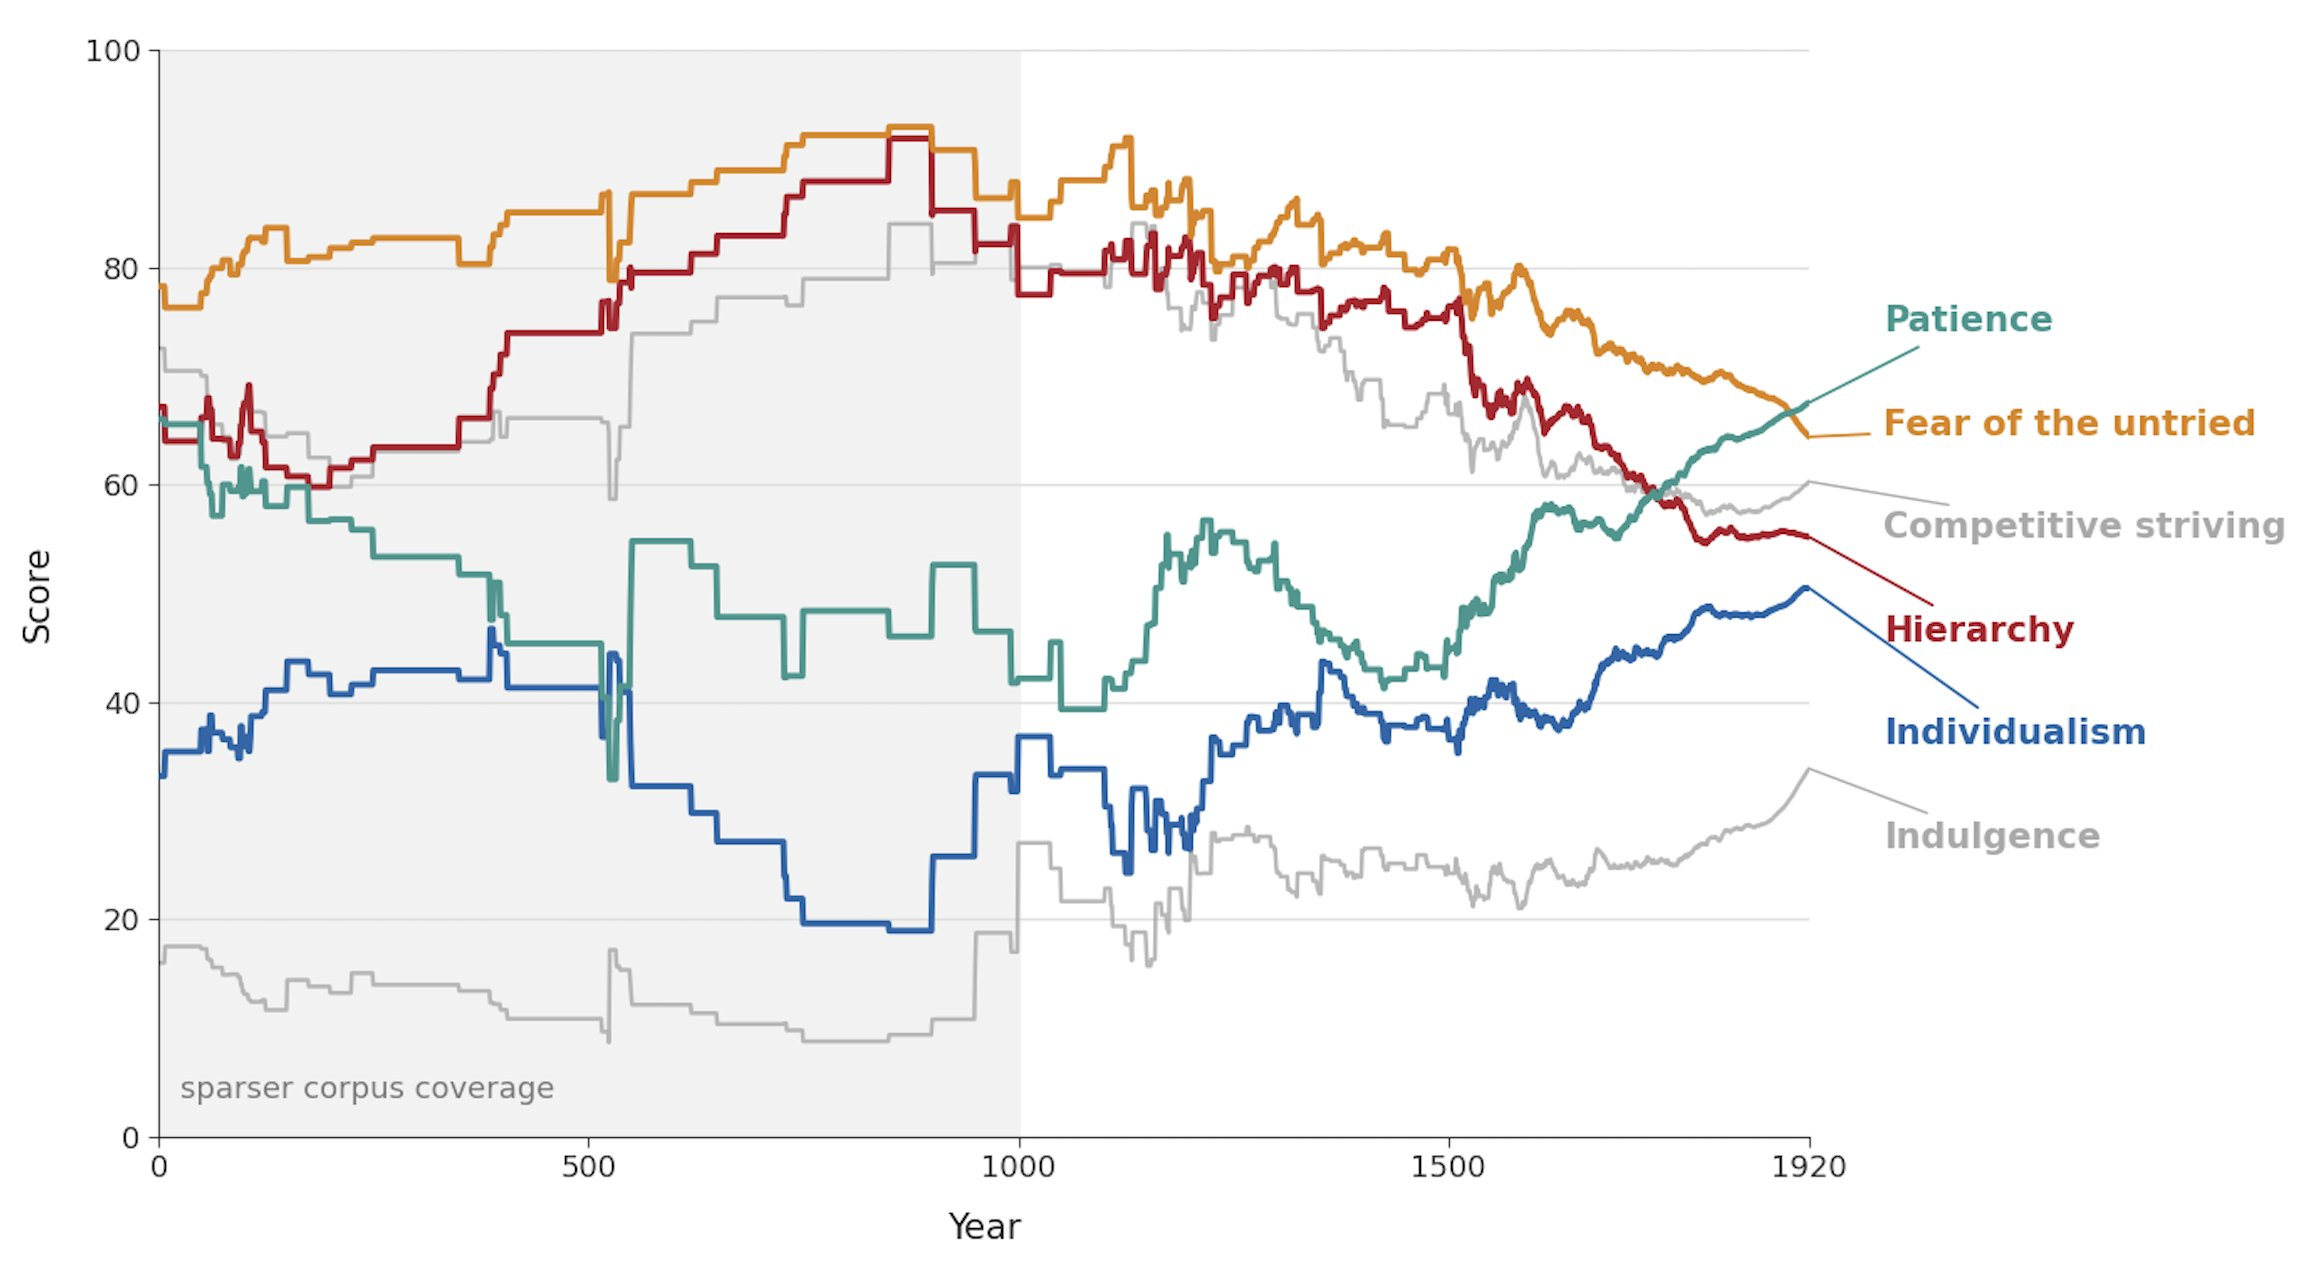
\includegraphics[width=\linewidth]{stefanski_culture_dimensions_0_1920.jpeg}

{\tiny\textit{Six dimensions, year 0--1920. The shaded pre-1000 band is sparser corpus coverage --- shown for direction only, not for inference.}}
\end{column}
\end{columns}
\smallskip
\textit{\footnotesize Source: Stefanski (2026), ``Cultural Capital and the Productivity of Ideas: Evidence from Historical Texts,'' Univ.\ of St Andrews Economics Discussion Paper No.~2602. Figure reproduced with attribution.}
\end{frame}

%=============================================================================
\begin{frame}{Why It Passes the T1 Bar}
\textbf{The EPU frame set the standard: audit every step. This case meets it with a different machine.}
{\footnotesize
\begin{itemize}
\item \textbf{Validation.} Experts \emph{blinded} to the scores agree with the score-implied direction in \textbf{93.0\%} of anchor comparisons among books they know; the stocks reproduce cross-country orderings from modern surveys; and an \textbf{independent 5{,}000-book archive} on a frozen pipeline reproduces the decline.
\item \textbf{The DGP, instantiated.} In $x_i = g(s_i, a_i, c_i) + \varepsilon_i$: $s_i$ is the work's stance; $a_i$ the authorial framing --- a satire \emph{depicts} what it does not endorse, which is why the scale needs a ``depicts'' category and a dictionary cannot supply one; $c_i$ is the archive.
\item \textbf{What it buys.} The falling wedge raises 1920 productivity to \textbf{1.78$\times$} its counterfactual level, explains \textbf{two-thirds} of the first sustained growth acceleration (1500--1700), and accounts for \textbf{38.7\%} of 1920 productivity growth --- culture as a \emph{measured series}, not a residual.
\end{itemize}}
\begin{cautionbox}
{\footnotesize \textbf{$c_i$ binds here.} The corpus is \textbf{``selected twice''}: history chose what was preserved and taught; digitizers chose which survivors were scanned. The first selection is part of the object of study --- the second is not, and no amount of model quality repairs it.}
\end{cautionbox}
\smallskip
\textit{\footnotesize Cost drove the architecture: Gemini~2.5~Pro runs the context pass once per book, Flash the passage stages that run hundreds of thousands of times.}
\end{frame}

%=============================================================================
\begin{frame}{China Parallel: The Same Method on Chinese History}
\textbf{The method is not about the West --- it is about any canon large enough to read and dated well enough to index.}
{\footnotesize
\begin{itemize}
\item \textbf{Corpora already digitized:} the Twenty-Four Histories; the \emph{Siku Quanshu}; local gazetteers (\emph{difangzhi}) --- thousands of volumes at fine geographic resolution; Ming--Qing memorials and legal archives; examination essays; clan genealogies; \emph{Shenbao} (1872--1949) for the late period.
\item \textbf{The question it could reach.} The Needham puzzle and the Great Divergence turn on cultural claims --- attitudes to hierarchy, novelty, the long horizon --- argued narratively because no series exists. The same scoring would put a Chinese series beside the Western one and let the growth model arbitrate instead of the anecdote.
\end{itemize}}
\begin{cautionbox}
{\footnotesize \textbf{What breaks --- and this is the point of the exercise.}
\begin{itemize}
    \item \textbf{Selection is stronger here, not weaker.} Imperial editorial projects did not merely preserve --- the \emph{Siku Quanshu} suppressed and altered as it collected. $c_i$ is partly a \emph{censorship} process, correlated with the very attitudes to authority being measured.
    \item \textbf{Register drift.} Classical and vernacular coexist for centuries; the same characters shift meaning across them.
    \item \textbf{Segmentation is itself a modeling decision}, before any scoring (Act~2).
    \item \textbf{Hofstede's dimensions were built for modern survey respondents.} Porting them to an imperial canon is an assumption needing its own blinded anchor study --- the 93\% exercise, repeated with Sinologists.
\end{itemize}}
\end{cautionbox}
\end{frame}

%=============================================================================
\section{Preview: The Machine Ahead}
\sectiondivider{Preview: The Machine Ahead}{One equation will power everything in Acts 2--4}

\begin{frame}{A Brief History: RNN $\rightarrow$ Transformer $\rightarrow$ GPT}
\begin{itemize}
\item \textbf{2003:} Bengio et al. neural language model --- continuous word vectors
\medskip
\item \textbf{2013:} Mikolov et al. \emph{Word2Vec} --- dense word embeddings at scale
\medskip
\item \textbf{2014:} Pennington et al. \emph{GloVe} --- global co-occurrence matrices
\medskip
\item \textbf{2017:} Vaswani et al. \emph{``Attention Is All You Need''} --- the Transformer replaces RNNs/LSTMs
\medskip
\item \textbf{2018:} Devlin et al. \emph{BERT} (encoder); Radford et al. \emph{GPT} (decoder)
\medskip
\item \textbf{2020--2022:} GPT-3, instruction tuning, RLHF $\rightarrow$ ChatGPT moment
\medskip
\item \textbf{2023--2026:} GPT-4/5, Claude (3--4), Gemini, LLaMA-3, DeepSeek; long-context (100k--1M tokens), open-weights ecosystem, agentic systems
\end{itemize}

\medskip
\textbf{Driver of the shift:} attention scales better than recurrence, both in compute (parallel) and in quality (long-range dependencies).
\end{frame}

\begin{frame}{The Autoregressive Principle}
\begin{itemize}
\item An LLM is fundamentally a \textbf{next-token predictor}:
\[
   p\bigl(t^{(n+1)} \mid t^{(1)}, t^{(2)}, \ldots, t^{(n)}\bigr).
\]

\medskip
\item \textbf{Generation:} sample $t^{(n+1)}$ from this distribution, append to the context, and repeat.

\medskip
\item \textbf{What this single equation enables} (the full revisit comes at the end of Act 4, once pretraining and fine-tuning are on the table):
\begin{itemize}
    \item \textbf{Summarizing 10-K filings or FOMC minutes} --- prompt with document + instruction; the model predicts summary tokens one by one
    \item \textbf{Generating narrative forecasts} conditional on macro state --- condition on data in the prompt; next tokens extend the narrative
    \item \textbf{Producing scenario analyses in plain language} --- the scenario is the context; prediction fills in the implications
    \item \textbf{Writing and debugging code} for empirical work --- same objective over a code corpus yields code completions
\end{itemize}

\medskip
\item \textbf{Key insight:} ``everything is next-token prediction'' is mathematically tiny but pedagogically and practically enormous.
\end{itemize}
\end{frame}

\end{document}
